\documentclass[12pt]{article}
\usepackage[letterpaper, portrait, margin=1in]{geometry}
\usepackage{authblk}
\usepackage[style=alphabetic,backend=biber]{biblatex}
\addbibresource{./sources.bib}

\input{/Users/sidbaskaran/preamble.tex}

\lstset{
	basicstyle=\ttfamily\scriptsize,
	frame=single,
	breaklines=true,
	mathescape,
    numberstyle=\color{gray},
    stringstyle=\color[HTML]{933797},
    commentstyle=\color[HTML]{228B22},
    emph={[2]from,import,pass,return}, emphstyle={[2]\color[HTML]{DD52F0}},
    emph={[3]range}, emphstyle={[3]\color[HTML]{D17032}},
    emph={[4]for,in,def}, emphstyle={[4]\color{blue}},
    showstringspaces=false,
    prebreak=\mbox{{\color{gray}\tiny$\searrow$}},
    numbers=left,
    xleftmargin=15pt
}

\hypersetup{
    colorlinks,
    citecolor=black,
    filecolor=black,
    linkcolor=black,
    urlcolor=black
}
\urlstyle{urlcolor=blue}

\title{Personal Finance Project}
\author[1]{Sidharth Baskaran}
\author[1]{Hamzah Rasool}
\affil[1]{Liberal Arts and Science Academy}
\date{March 29, 2022}

\begin{document}
\maketitle

\tableofcontents
\newpage

\section{Overview}

\textit{Project typesetting and Python source code repository}: {\color{blue} github.com/sidnb13/personal-finance}.

Jeff is the simulated person this financial plan is made for. Jeff is currently a 25-year-old college graduate with no student debt and lives in Albuquerque, New Mexico. He landed a decent full-time job with a salary of \$55,000 a year taxed at 30\% with a 1\% increase in salary every year. Jeff, intelligently, is already thinking about financial independence and planning for retirement. Through frugal housing, utilities, transportation, food, entertainment, and clothing spending along with consistent, safe investing in a Roth IRA, Jeff will be able to comfortably retire at the age of 68 with well over \$2.5 million in personal wealth.

In the United States, it is a common trend for those with lower incomes to remain in that standard of living
due to an inability to save--the emphasis is placed on survival and short-term growth over long-term well-being of one and their family's future.
With this new proposal, the objective is to draft a realistic and attainable plan
to amass significant residual wealth while relying on a modest income and a frugal expenditure lifestyle.
The general approach to our financial plan involves framing our post-tax annual income expenditure primarily around
low-risk investment techniques: namely a Roth IRA account and a Series I Savings Bond, to which annual contributions are maxed-out.

Furthermore, we aim to purchase a very conservative number shares annually in high-risk sectors such as stocks
of well-known technology corporations and promising startup industries. Taking this approach, we
primarily rely on reliable investments while taking the benefits of high-risk investments, but with minimal risk.
In regards to personal expenditures necessary for a modest lifestyle, we propose to limit expenditures on luxury items
and aim to purchase used items wherever necessary, for they minimize loss when taking into consideration
capital investments with large depreciation (i.e. motor vehicles).

Due to the high financial barrier of
entry to real estate, we aim to simply purchase a modest home when our savings afford a cash purchase.
Given that we utilize two low-risk investment vehicles, the excess wealth exceeding \$2.5 million will
safely allow this expenditure among others.

For the purpose of this study, we base simulations and cost-of-living estimates in Albequerque, New Mexico.
We utilize the tax rate of 30\% for all taxable accounts and do not account for sales tax on purchases for simplicity.
We will also utilize the 1\% inflation rate for the purchase of personal essentials.

\section{Contingencies}

In order to plan for contingency events, we propose to maintain the required \$55,000 emergency
fund throuhout the simulated lifetime of 25 to 68 years. By age 30, this fund will be established
by equal installments over each of the 5 years. After this, a smaller annual amount will be incrementally contributed to augment its growth.
In order to harness the power of compounding and minimize risk, we will utilize a high-yield investment account
paired with a savings account \cite{SavingAcc}. In the first five years, we contribute aggressively to each account in equal portions of \$5500.
Thus, disregarding interest we will end up with a base salary's worth of \$55000 in the emergency fund in 5 years.
The added returns will count as padding for volatility in markets.

\begin{enumerate}
    \item A savings account will be opened, and \$5500 will be contributed annually.
    We will utilize the Marcus savings account by Goldman Sachs \cite{SavingAcc}, which provides an annual percentage yield (APR) \cite{SavingAcc} of 0.5\%.
    \item Likewise, \$5500 will be invested into the S\&P 500 index fund annually.
\end{enumerate}

Note that we will not utilize an untaxed Roth IRA for the emergency fund in order to avoid the 10\% penalty for an unplanned withdrawal \cite{RothIra}.
After running the simulation for 5 years, our aggressive split-stock and saving strategy results in \$55952 of emergency funds within the first 5 years.

\section{Personal Expenditures}

Our personal expenditures will be categorized into monthly living expenses (e.g. rent, utilities, subscriptions, life insurance) and one-time purchases (e.g. car, house).
Analagous to our Python simulation, we will set "breakpoints" for these payments at the expected time that they will be paid off.
For example, we stop paying rent for our studio apartment after we build/move into the house. Below is an exhaustive set of tables of our annual-totaled expenditures, automatically generated by the Python script \cite{car}\cite{mortgate}\cite{EmFund}.

\begin{center}
    \begin{center}
        \begin{tabular}{|l|c|c|c|c|}
                \hline
                \textbf{Item} & \textbf{Cost} & \textbf{Start} & \textbf{End} & \textbf{Period} \\
                \hline
                Food & 150 & 2022 & Indefinite & monthly \\
                \hline
                Rent & 540 & 2022 & 2025 & monthly \\
                \hline
                Utilities & 140 & 2022 & Indefinite & monthly \\
                \hline
                Life insurance & 15 & 2022 & Indefinite & monthly \\
                \hline
                Mortgage & 730 & 2042 & Indefinite & monthly \\
                \hline
                Gas & 550 & 2025 & Indefinite & yearly \\
                \hline
                Car insurance & 950 & 2025 & Indefinite & yearly \\
                \hline
                Roth IRA contrib & 500 & 2022 & Indefinite & monthly \\
                \hline
                Savings account contrib & 5500 & 2022 & Indefinite & yearly \\
                \hline
                Bond purchases & 11000 & 2027 & Indefinite & yearly \\
                \hline
                Stock share purchases & 5500 & 2022 & Indefinite & yearly \\
                \hline
                Down payment & 4875 & 2026 & 2026 & yearly \\
                \hline
                Car purchase & 7500 & 2025 & 2025 & yearly \\
                \hline
        \end{tabular}
\end{center}
\end{center}

Note the staggered strategy of paying for the car and house down payments as soon as possible. 
Jeff bought a car. He wanted to purchase one after he had keys to his house so his mortgage loan would be approved as applying for a car loan can temporarily reduce your score. 
He bought a 2007 Toyota Avalon for a total payment of \$4875 plus \$950 for auto insurance annually \cite{car}. Gas costs him \$450 annually as well.
Thankfully, the venerable Toyota is quite fuel efficient and reliable, making this a consistent yearly fixed price and the car happily survives with Jeff without need of a single maintenance check-up.
Once Jeff is comfortably settled into his studio apartment, he becomes agressive and purchases a down payment on his dream Albequerque getaway and the Avalon he's been eyeing for a few years now.
With these major purchases out of the way, Jeff now aims to purchase a healthy investing of bonds which we will discuss in the next section while he starts smartly paying his mortgage.
With around 39 years of a low mortgage payment, Jeff will end up owning a house worth \$351000.

In terms of general insurance (vision, dental and primary care), Jeff is fully covered and can get the care he needs if necessary. His plan is the Ambetter Essential Care 2 HSA + Vision + Adult Dental \cite{insurance}. The monthly rate for this plan is \$290.45. 
Annually he spends about \$3,485.40. Once Jeff turned 65, he wanted a different plan because of his age and his plans to retire soon. He didn't qualify for a retiree's health plan because he was still working, but he wanted a plan with better coverage for seniors. So he opted for Medicaid as his new health care plan, costing him \$0.
He pays around \$15 a month for Allstate life insurance as well \cite{lifeinsurance}.

There is residual or excess income following all of these expenditures at the end of each year. Jeff, being a philanthropic and selfless man of his values, donates every remaining penny to the UNICEF organization.

\section{Investments}

The vehicles of investment Jeff ends up using are Series I Savings Bonds (taxed), a Roth IRA retirement account (untaxed), and an investment account where he solely buys shares of S\&P 500 index fund.
As mentioned before, the sum of asset worth in the saving and stock accounts represents the emergency fund, of which we satisfy the minimum requirement after 5 years and then utilize its power as an investment vehicle.
Series I Savings Bonds offer the benefit of being immune to the volatility of the stock market; therefore they are low-risk investment vehicles. Furthermore, the Roth IRA retirement account is non-taxed on its returns
but also maintains a 10\% withdrawal fee prior to retirement, so Jeff will be incentivized to actually use this money for retirement \cite{RothIra}.
In the below Python-generated graphic, we can see the timeline-based results of Jeff's investment portfolio.

\begin{figure}[H]
    \centering
    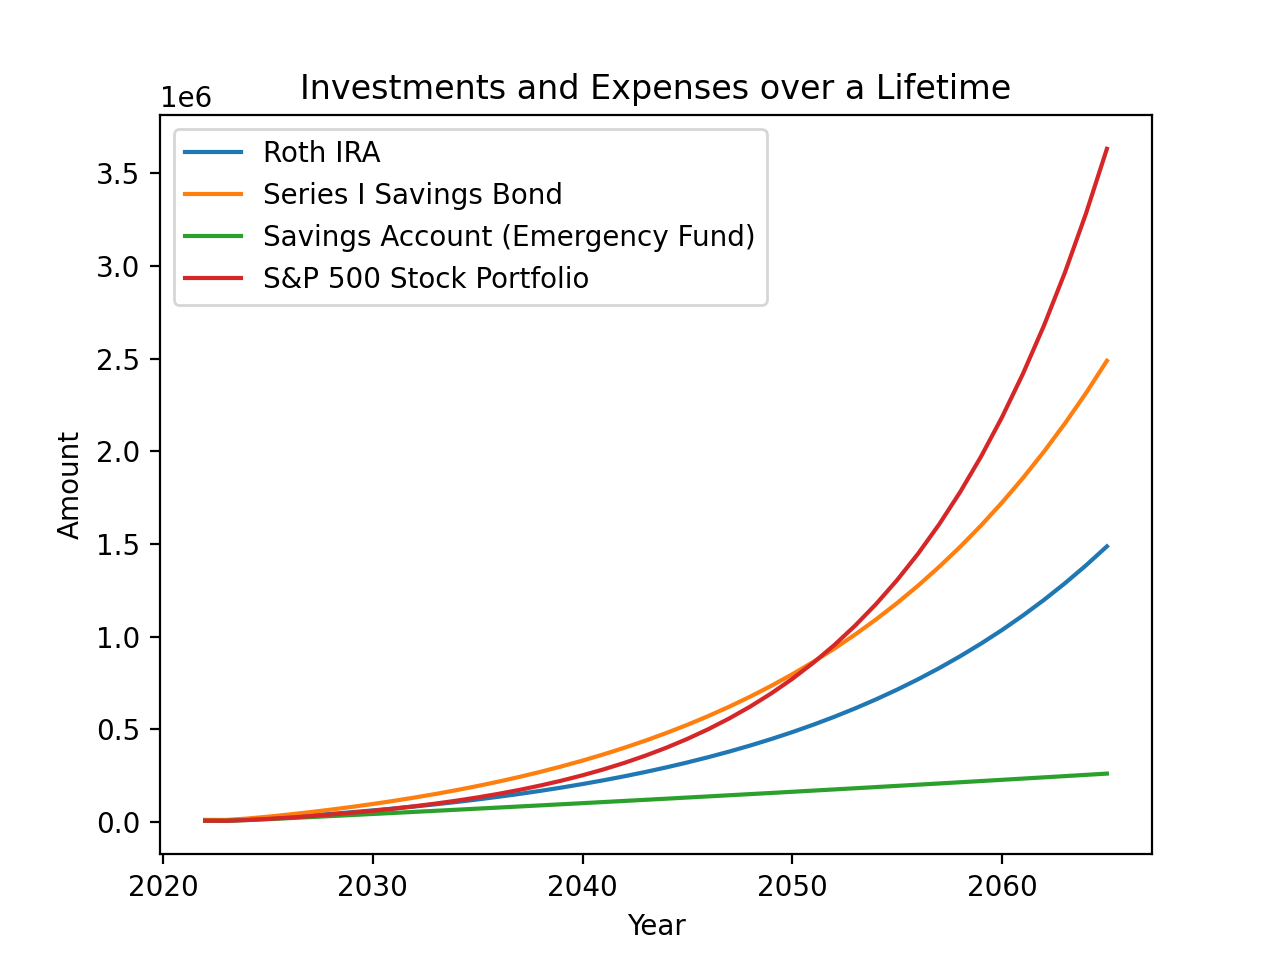
\includegraphics[scale=0.75]{wealth.png}
    \caption{Investment portfolio over time}
\end{figure}

We observe an easy way to calculate compounding investments for a general portfolio. This is very important to the way in which we calculated our portfolio over time and made the best estimates.
Say we contribute $P$ to the portfolio every year indefinitely and the vehicle has a return rate $r$, compounding annually. Let the year be $t=0$.
In the first year we have $Pr^0=P$, and the second year $P+Pr$. We keenly identify this as a geometric progressive sum with common ratio $r$.
First, factor out $P$ and apply a series of algebraic manipulations to obtain the portfolio's value at any given $t$. (Let us desire the value at $t=n$ years)
\begin{align*}
    A_n &= P\left(r^{n-1} + r^{n-2} + \ldots + 1\right)\\
    rA^n&=P\left(r^{n} + r^{n} + \ldots + r\right)
\end{align*}
Then,
\begin{align*}
    A_n(r-1)&=P\left(r^{n}-1\right)\implies A_n=\frac{P\left(r^{n}-1\right)}{r-1}
\end{align*}

This basis is very flexible, and we can apply taxable gains easily. Let $A_n$ be the current portfolio at the end of year $n$
and $A_{n-1}$ represent the value at the end of the previous year, resulting in return of $A_n-A{n-1}$. Applying a tax rate $R$,
we get the tax-adjusted portfolio value to be $A_{n-1} + R(A_n-A_{n-1})$.

\newpage
\section{Python Simulation}

\lstinputlisting[language=Python]{./calculate-expenditure.py}

\section{Conclusion}

By the time Jeff retires at age 68, he will have amassed  over \$7.8 million in personal wealth. 
His Roth IRA returned \$1.48 million with bonds cashed in for \$2.48 million, and stock portfolio of \$3.6 million with \$260217 in his savings account. He was able to live comfortably and securely in Albuquerque, New Mexico. 
With no wife or children, Jeff will live in peace and prosperity.

\newpage
\printbibliography

\end{document}